\documentclass[letterpaper]{article}

\usepackage{outline}
\usepackage{graphicx}
\usepackage{listings}

\lstset{numbers=left, basicstyle=\footnotesize}

\begin{document}

\title{Implementing Distributed Systems Directly with I/O Automata in Ioa++}
\author{Justin R. Wilson \and Christopher D. Gill}
\date{}

\maketitle

\begin{abstract}
The ability to realize sophisticated distributed reactive systems such as those found in cyber-physical or pervasive computing environments is predicated on a suitable model and implementation of asynchrony and concurrency.
The size and complexity of these systems implies that software re-use in their development, maintenance, and evolution is also essential.
Taken together, these requirements demand appropriate programming abstractions through which different forms of asynchrony and concurrency can be realized directly in reusable software.
To that end, this paper presents the ioa++ framework for developing distributed reactive systems, which is the primary contribution of this research.
We develop a component model in which the asynchrony and concurrency of reactive distributed systems can be represented naturally based on I/O automata and dynamic composition.
We describe the design and implementation of that component model in ioa++ and illustrate its use in developing a prototype distributed coordination protocol.
We also evaluate concurrency performance in ioa++ through a series of micro-benchmarks which confirm that the framework’s ability to exploit potentially concurrent execution is limited only by the interactions of the automata that comprise the system and the overhead of synchronization.

\keywords{concurrency, I/O automata, components}
\end{abstract}

%% \begin{abstract}
%% The ability to realize sophisticated distributed systems such as those found in cyber-physical, pervasive, or enterprise computing environments is predicated on a suitable model and implementation of asynchrony and concurrency.
%% The size and complexity of these systems implies that software re-use in their development, maintenance, and evolution is also essential.
%% Taken together, these requirements demand appropriate programming abstractions through which different forms of asynchrony and concurrency can be realized directly in reusable software.
%% % By ``different forms'' we mean single-threaded, multi-threaded, time triggered, event triggered, etc.

%% To that end, this paper presents the \emph{ioa++ framework} for developing distributed systems, which is the primary contribution of this research.
%% We develop a component model for asynchronous and concurrent systems based on I/O automata and dynamic composition.
%% We describe the design and implementation of the component model in ioa++ and show how it can be used to develop protocols and other forms of distributed software.

%% Our experiences demonstrate that ioa++ can help simplify developing distributed systems, by supporting reasoning about asynchronous and concurrent programs directly from source code using the I/O automata formal model.
%% Common concurrency and interaction semantics allow simple modules to be aggregated into complex systems without building adapters that convert from one concurrency model to another.
%% % I've just commented this out instead of trying to weave it in elsewhere, especially since I think it is already somewhat implied by the threads discussion in the intro - Chris
%% %Whereas reasoning about the correctness of modules in a threaded program requires considering interactions among the various threads, reasoning about the correctness of modules in ioa++ is limited to the modules themselves and a well-defined set of composition rules.

%% We evaluate concurrency performance in ioa++ through a series of micro-benchmarks which confirm that the framework's ability to exploit potentially concurrent execution is limited only by the interactions of the automata that comprise the system and the overhead of synchronization.
%% \end{abstract}


\section{Introduction\label{introduction}}

Advances in platforms and networks are paving the way for distributed reactive systems of unprecedented sophistication.
Cyber-physical systems go beyond the traditional embedded system paradigm by explicitly integrating the dynamics of the physical system in the computational task.
Pervasive computing environments are emerging in our homes, offices, and hospitals as more and more devices are equipped with wireless network interfaces.
The interactions these systems have with the physical environment, communities of users, and each other, require a degree of interoperability, configurability, adaptability, scalability, robustness, and security not readily supported by existing approaches.

In particular, the activities performed by such reactive distributed systems are intrinsically concurrent and asynchronous.
Nodes sense and manipulate the environment and interact with other nodes by sending and receiving messages.
To produce more sophisticated systems with current levels of effort, we wish to construct \emph{correct} systems by \emph{composing} modules whose execution is concurrent and asynchronous.
The ease with which asynchronous and concurrent modules can be \emph{developed} and \emph{reused} is thus essential.
Modularity, well-defined interfaces, and rigorous composition rules are also crucial to facilitate reasoning about the interactions among system components and to allow a group of interacting components to be understood as a cohesive unit.

\paragraph*{Limitations of the state of the art.}
Existing component frameworks are often implemented using threads, event loops, or a combination of both.
We limit our scope to imperative frameworks but note that functional approaches are also gaining popularity~\cite{armstrong1996concurrent},~\cite{halloway2009programming}.
Although threads provide a natural synchronous sequential processing model, the difficulties of using threads in practice are well known~\cite{lee2006problem},~\cite{sutter2005free}.
For example, a component that doesn't acquire locks in the same order as others may cause deadlock~\cite{havender1968avoiding}.
Event loops execute handlers in response to external (I/O) and internal events and have been proposed as a simpler alternative to threads~\cite{ousterhout1996threads}.
However, that approach lacks common semantics for how events are generated, distributed, and consumed; thus complicating composition.
\emph{A key challenge, then, is to provide a component framework for programming asynchronous and concurrent systems that avoids the complications of thread-based development while providing common event semantics and opportunities to exploit concurrent execution.}

\paragraph*{Contributions of this work.}
To address this challenge we present the ioa++ framework for building distributed reactive systems, which is based on the I/O automata formal model. 
This paper makes three main contributions to the state of the art:
(1)  a model for \emph{dynamic} systems of I/O automata which is necessary for implementing (as opposed to only modeling) many distributed systems,
(2)  a C++ implementation of the model that allows one to build real systems using the facilities provided by POSIX environments, and
(3)  a preliminary investigation into the degree of \emph{exploitable concurrency} in a system as a function of the automata interactions and framework overhead.
The ioa++ framework is freely available as open-source at \url{http://jrwilson.github.com/ioa/}.

%\paragraph*{Paper structure}
In Section~\ref{component_model}, we motivate I/O automata as a suitable foundation for components and introduce a model for dynamic systems.
Section~\ref{design} describes the design and implementation of the ioa++ framework and Section~\ref{programming_model} describes how component automata are programmed within it.
In Section~\ref{case_study}, we show how ioa++ can be used to build a simple but representative example of distributed software by implementing a leader election protocol for a ring of processes connected by TCP sockets.
We evaluate the ability of ioa++ to exploit potential concurrency with a series of micro-benchmarks in Section~\ref{evaluation}.
Section~\ref{related_work} summarizes related work and we offer conclusions in Section~\ref{conclusion}.

%% The component model behind our framework is based on our objectives for aysnchrony and concurrency tempered with a number practical considerations.
%% (1) Internally, components are imperative instead of functional.
%% A component is a set of state variables that are manipulated by assignment statements.
%% This matches existing machine architectures and popular languages such as C, C++, and Java.
%% (2) Components communicate with messages instead of reading and writing shared variables.
%% We observe that the auxiliary variables necessary to access shared variables correctly add unnecessary complexity.
%% Furthermore, the distributed systems we are targeting are based on message passing instead of shared memory and a component based on message passing can be integrated without an impedance mismatch.
%% (3) The state of one component is independent from another and components are structured as a set of atomic actions or events.
%% This obviates the need for primitive locks which are tedious and error-prone.
%% Events match the asynchronous and reactive nature of the targeted distributed systems.
%% (4) The concurrent execution of \emph{some} actions in different components should be possible.
%% Concurrent execution on multiple processor cores is the only foreseeable way to achieve increased levels of performance given the leveling of clock frequencies and the advent of multi-core technologies.
%% The atomicity of each action prohibits the concurrent execution of two actions in the same component while the independent state of each component implies that actions in different components can be executed concurrently.
%% We entertain the idea that some actions might not be capable of executing concurrently due to composition.
%% (5) Components can be configured to communicate with each other.
%% It must be possible for component $C$ to direct an output of component $O$ to an input in component $I$.
%% We call such a relationship a \emph{binding}.
%% %% This is analogous to connecting the pin of one electrical component to another with a wire.
%% Factoring the interaction into an output, a binding, and an input is important because it encourages modular designs with configurable communication.
%% (6) Communication among components will be unbuffered.
%% Unbuffered communication seems more fundamental as buffered communication can be implemented in terms of unbuffered communication but not vice versa.
%% Unbuffered communication and atomic actions imply that an output action in one component executes atomically with a bound input in another component.
%% This allows the state of communicating components to be correlated and facilitates composition.
%% (7) 

%% dynamics
%% backed by a formal model

%% The two main approaches to developing concurrent modules are threads and event handling.
%% Threads offer a seemingly straightforward extension of the synchronous sequential processing model supported by modern processors, programming languages, and operating systems.
%% Applications using threads are often structured for functional modularity, e.g., using the object-oriented paradigm where separate modules use one another to accomplish a computational task and locks are used to control concurrent access to each module.
%% The thread approach is typified by the synchronization, e.g., Strategized Locking, and concurrency patterns, e.g., Active Object, of~\cite{schmidt2000pattern}.

%% Developing concurrent modules with threads is difficult and the very nature of threads complicates composition.
%% The majority of threaded systems are developed with locks which is considered hazardous by industry~\cite{sutter2005free}.
%% In a position paper, Lee identifies that the difficulties encountered when using threads arise from the pairing of shared state and non-determinism~\cite{lee2006problem}.
%% Automated program analysis and verification techniques are often required to find and correct bugs in threaded programs.
%% One way to avoid deadlock when using multiple shared resources is for the threads to acquire the locks in order~\cite{havender1968avoiding}.
%% However, doing so would break encapsulation because of the need to know the recursive locking requirements for any used module.
%% The difficulty of identifying and evaluating the behavior and requirements of concurrent modules thus may inhibit the construction of truly reusable concurrent modules.

%% The event handling approach is typified by software engineering patterns like Reactor~\cite{schmidt2000pattern}, and Proactor~\cite{schmidt2000pattern}.
%% Event handling is based on a loop containing a call to an event multiplexer, e.g., an event loop, that dispatches registered event handlers.
%% Computation is structured as a set of event handlers that are invoked for the corresponding event.
%% Event handling is often a simpler alternative to threads, especially when true concurrent execution is not required~\cite{ousterhout1996threads}.

%% The event handling approach suffers from a problem that prevents composition that can summarized by the question:  ``Who has the event loop?''
%% To illustrate this issue consider the problem of providing a graphical user interface using Java Swing for a middleware based on the Reactor or Proactor design pattern~\cite{schmidt2000pattern}.
%% One solution involves running both event loops in independent threads and thus facing all of the challenges associated with multiple threads discussed previously.
%% The alternative is to either convert Java Swing to use the middleware's event loop or to convert the middleware to use Java Swing's event loop.
%% Composing two event systems thus requires a common definition of events and agreement upon how events are generated, distributed, and consumed, which is not often the case.

%% If we step back



%% Implementation matters.
%% You can't build a skyscrapper with toothpicks.

%% How are systems implemented in practice:
%% threads ->
%% event loops ->
%% actors ->

%% If we want a new ``brick'', what should it look like?
%% - Should resemble a formal model.  This helps even if we don't write proofs.
%% - The right level of abstraction.  Not two high, not too low.  Sometime we need to get down and dirty.
%% - Composition (fractal nature)
%% - Components
%% - Should resemble what we believe to be fundamental.

%% Formal models and their ability to produce new ``bricks'':






%% Advances in platforms and networks are paving the way for distributed systems of unprecedented sophistication.
%% Cyber-physical systems go beyond the traditional embedded system paradigm by explicitly integrating the dynamics of the physical system and communication network in the computational task.
%% Pervasive computing environments are emerging in our homes, offices, and hospitals as more and more electronic devices are equipped with wireless network interfaces.
%% Enterprise computing systems continue to grow in size, complexity, and diversity as businesses look for new ways to utilize their computing infrastructure to support client interactions and internal business processes.
%% The interactions these systems have with the physical environment, its community of users, and each other, require a degree of interoperability, configurability, adaptability, scalability, robustness, and security not readily supported by current system development approaches.

%% The activities performed by the nodes in the distributed systems we desire to build are intrinsically concurrent and asynchronous.
%% Nodes may continuously sense and manipulate the environment, perform background processing, and interact with other nodes by sending and receiving messages.
%% Often, the program running on a node will straddle multiple logically independent systems and participate in a number of protocols.
%% To achieve increasing degrees of sophistication with current levels of effort, we require the ability to construct programs by integrating a number of protocol-specific modules where each module itself is concurrent and asynchronous.

%% %% However, existing techniques for developing concurrent and asynchronous software modules do not match the semantics of distributed systems and fail to provide the degree of reusability necessary for developing sophisticated distributed systems.
%% %% The three techniques that are commonly used in practice are threads, communicating sequential processes, and events.

%% %% Distributed systems are built using threads by assembling a constellation of reusable thread-safe objects.
%% %% However, developing even simple thread-safe objects is difficult due to the pairing of shared state with the arbitrary interleaving of machine instructions~\cite{lee2006problem}.
%% %% Furthermore, the use of locks to control access to shared state complicates re-use as the locking requirements of each used module must be recursively understood to prevent currency hazards.
%% %% The inability to communicate and cope with arbitrary locking requirements and the general difficulty associated with developing thread-safe modules implies that threads are an inappropriate abstraction for building sophisticated distributed systems.

%% %% Distributed systems are built using communicating sequential processes by decomposing the problem into pieces of independent state manipulated by a sequential process and then configuring the processes to communicate using channels\footnote{For this discussion, we assume that processes that communicate using multiple channels have at least two rendezvous points to distinguish communicating sequential processes from events.}.
%% %% The sequential nature of communicating sequential processes forces a deterministic and synchronous interpretation of inherently non-deterministic and asynchronous problems.
%% %% For example, the arrival of a sensor reading in relation to network messages is often irrelevant but the developer is forced to choose an order for these activities.
%% %% Artificially ordering communication can introduce concurrency hazards when communicating sequential processes are assembled to form complex systems, e.g., a deadlocking system might reduce to process A expecting to read channel 1 and then 2 while process B expects to write channel 2 and then channel 1 when the nature of problem makes the order in which the channels are read irrelevant.

%% % Core Issues
%% %% One of the forces that complicates the development of any kind of sophisticated software system is accidental complexity~\cite{brooks1987no}.
%% %% Accidental complexity stems from a mismatch between the semantics of the conceptual model and semantics of the implementation method introduces errors and slows development as developers are constantly switching from one set of semantics to the other.
%% %% While there is no ``silver bullet''~\cite{brooks1987no}, reducing accidental complexity increases productivity and makes new levels of sophistication possible with existing levels of effort.

%% %% In the context of distributed systems, a major source of accidental complexity is the mismatch between the asynchronous semantics of distributed systems and the synchronous techniques used to implement them.
%% \paragraph*{Limitations of thread models}
%% Threads are the \emph{de facto} standard concurrency mechanism for many distributed systems.
%% Threads offer a seemingly straightforward extension of the synchronous sequential processing model supported by modern processors, programming languages, and operating systems.
%% While the widespread availability of thread libraries makes them a natural choice for system development, using threads to develop distributed systems has significant drawbacks.

%% % Illustrate the problem
%% First, developing concurrent programs with threads is difficult.
%% Lee identifies the source of this difficulty as the pairing of shared state with the non-deterministic interleaving of machine instructions~\cite{lee2006problem}.
%% The properties that make the synchronous sequential model of computation useful for developing programs, i.e., ``understandability, predictability, and determinism''~\cite{lee2006problem}, are lost with the immediate introduction of non-determinism.
%% After introducing non-deterministic execution with threads, programmers must ``prune''~\cite{lee2006problem} the portions of the resulting reachable state space to remove execution sequences that result in bad states.
%% Identifying all possible paths to bad states is sufficiently challenging that automated program analsysis and verification techniques are often required to find and correct such errors.

%% %% [Additional fodder.]
%% %% First, threads are difficult to treat formally and therefore \emph{very} difficult to treat informally.
%% %% The correctness of programs is reasoned about either formally as part of formal software design and verification and/or informally during the debugging process.
%% %% Since most programs will never be formally verified, the correctness of most programs hinges solely on the developers ability to reason about the program.
%% %% Based on the historical example of structured programming~\cite{goto_considered_harmful}, there is a strong correlation between what is ``easy'' in the formal arena and what is ``easy'' in the informal arena, especially when the implementation mimics the formal model, e.g., structured programming languages.
%% %% It is well known that a formal treatment of threads is difficult due to the arbitrary interleaving of critical sections and the ability to define critical sections of arbitrary scope~\cite{lee_threads}.
%% %% Thus, the correctness of most multi-threaded programs hinges on the developer's ability to explore arbitrary interleavings of critical sections, i.e., model checking, in their head.

%% Second, the lack of a common standard calculus for controlling access to shared state variables inhibits the development of reusable software modules.
%% Applications using threads are often structured for functional modularity, e.g., using the object-oriented paradigm where separate modules use one another to accomplish a computational task and locks are used to control concurrent access to each module.
%% One way to avoid deadlock when using multiple shared resources is for the threads to acquire the locks in order~\cite{havender1968avoiding}.
%% However, doing so would break encapsulation because of the need to know the recursive locking requirements for any used module.
%% The difficulty of identifying and evaluating the behavior and requirements of concurrent modules thus may inhibit the construction of truly reusable concurrent modules.

%% %% [Additional fodder.]
%% %% Second, the lack of a standard calculus for threads prevents developing reusable software modules.
%% %% To illustrate this problem consider the challenge of developing an application with a graphical user interface that also uses a multi-threaded middleware library.
%% %% Graphical user interfaces often use a single-threaded event-based design, e.g., X, Swing.
%% %% The system integrator must write glue code that bridges the single-threaded event-based semantics to multi-threaded semantics.
%% %% Bridging between two thread models is achievable, however, the systems we desire to build will rely on many libraries each with their own thread model.
%% %% The importance of a unified approach to concurrency becomes apparent when one considers bridging between different threading models, e.g., event-based, reactor, proactor, active objects, and their attributes, e.g., thread creation, blocking vs. non-blocking I/O.

%% %% The decision to use threads stems from a desire to support multiple concurrent activities.
%% %% Threads are a good choice if the problem is embarrassingly parallel and necessary if one wishes to achieve true CPU concurrency, e.g., high performance computing.
%% %% To support multiple concurrent activities without threads, the different tasks are encoded as event handlers.
%% %% A single thread then waits for the events and dispatches the appropriate handler.
%% %% The illusion of concurrency, then, is accomplished by interleaving event handlers for different tasks.

%% \paragraph*{Limitations of event models}
%% Events~\cite{lamport1978time}, \cite{manna1992temporal} are a good choice for developing distributed systems due to their reactive semantics and support for asynchrony.
%% A node in a distributed system senses and actuates its environment and sends and receives messages to communicate with other nodes.
%% The input activities, sensing and receiving, are naturally asynchronous, i.e., they can come from the environment at any time.
%% The output activities, actuating and sending, in their most general form are also asynchronous as the environment might not be able to immediately consume data produced by a node.
%% Distributed systems are often specified as reactive state transition systems which map cleanly into events; transitions are encoded as event handlers and conditions which trigger a transition are encoded as events.

%% While events more closely match the semantics of distributed systems, the lack of a common standard calculus for events prevents the development of reusable software.
%% To illustrate this issue consider the problem of providing a graphical user interface using Java Swing for a middleware based on the Reactor or Proactor design pattern~\cite{schmidt2000pattern}.
%% One solution involves running both event loops in independent threads and thus facing all of the challenges associated with multiple threads discussed previously.
%% The alternative is to either convert Java Swing to use the middleware's event loop or to convert the middleware to use Java Swing's event loop.
%% Composing two event systems thus requires a common definition of events and agreement upon how events are generated, distributed, and consumed, which is not often the case.
%% % Continuous vs. halting. (search reactive systems, Amir Pnueli, Zohar Manna)

%% \paragraph*{Motivation for I/O automata}
%% It is thus clear that existing concurrency abstractions are inadequate to the needs of many sophisticated distributed systems and new approaches must be pursued.
%% While threads match the semantics of widely available synchronous processors, thread-based development may introduce hazards for the distributed system developer including obscure race conditions, poor support for asynchrony, and difficulties integrating software developed using different thread models.
%% Events, while matching the semantics of distributed systems more closely, are often inflexible, ad hoc, and lack a standard calculus to facilitate the creation of reusable event-based modules.
%% Alternative concurrency abstractions that more closely match the semantics of distributed systems \emph{and} facilitate software re-use are therefore needed.
%% % We aren't saying I/O automata are the best, just better than threads.

%% % Can we give an example?
%% %% Third, threads are ill-suited for the asynchronous semantics present in the systems we desire to build.
%% %% The distributed systems we desire to build are asynchronous at both the device and network levels.
%% %% Embedded devices must respond to asynchronous events in the environment.
%% %% The interrupt-driven TinyOS operating system for wireless sensor network motes is an exemplar in this area.
%% %% The fundamental communication primitive in real-world distributed systems is asynchronous message passing.
%% %% Realizing asynchrony in a threaded program requires the use of signals (interrupts) and/or (a)synchronous I/O multiplexing.
%% %% Signals are primitive, rigid, and difficult to use correctly.
%% %% Synchronous I/O multiplexing, e.g., a select loop, is limited to operating system abstractions, e.g., file descriptors, and induces a reactive state machine structure that is difficult to understand and maintain.
%% %% Asynchronous I/O improves efficiency by avoiding the dispatching necessary to determine the I/O operation but are subject to the same limitations of shared-state thread-based programming.

%% % This starts to got a bit far afield from the core points you're making, and probably should be (1) moved to the related work section and (2) replaced with a brief transition (a sentence or 2) in part D which outlines the contributions of the work.
%% %% Difficulties in developing asynchronous and concurrent software using threads has prompted a number of concurrent programming languages, e.g., Esterel, Erlang, Ptolemy, Autopipe, and language extensions, e.g., OpenMP, Cilk, Split-C.
%% %% Solutions that involve creating a new language or extending an existing language suffer from two main problems.
%% %% First, such solutions are often domain-specific and do not generalize to different applications, a necessity for heterogeneous distributed systems.
%% %% Furthermore, solutions not connected to a general-purpose formal model lack the important property that the complete system including the environment can be modeled as another component.
%% %% Second, such solutions often fail to become mainstream due to practical considerations.
%% %% For example, the combination of C and pthreads is much more popular than Erlang due to the popularity of C-like languages and C's connection with UNIX operating system.
%% %% Most language extensions are targeted at niche markets and therefore never standardized and implemented in mainstream compilers.

%% The reactive semantics of the I/O automata model match the asynchronous and concurrent semantics of distributed systems well and have been proven effective in the formal design and verification of real world distributed systems.
%% The I/O automata model prohibits shared state and thus avoids the problems stemming from it.
%% Furthermore, its precise semantics for composition facilitate the creation of reusable event-based modules that may be executed with different degrees of concurrency as we demonstrate in our evaluation presented in Section~\ref{evaluation}.
%% However, there is to date insufficient experience \emph{building} and \emph{evaluating} real distributed systems directly atop I/O automata.
%% Previous efforts in this area have focused mainly on formal software development, i.e., automata are described in a language suitable for theorem proving and simulation and afterward are translated into a production language for deployment\footnote{TODO:  Add citations.}.
%% The translation from modeling language to production language complicates interfacing with system facilities and makes developing low-level protocols difficult, an area which could greatly benefit from the direct application of I/O automata.
%% % Before giving the paper structure, needs to say (1) what the main contributions of the paper are, and (2) how the help address the challenges raised earlier in the intro
%% % Thus, in order to build sophisticated distributed systems, we require a common semantics and model for building concurrent and asynchronous systems with straight-forward abstractions.

%% \paragraph*{Paper structure and contributions}
%% This paper presents ioa++, a framework for building asynchronous and concurrent systems that is based on the I/O automata formal model.
%% %% The model must be general to support the wide variety of devices and protocols necessary for cyber-physical and pervasive computing systems.
%% %% The model must facilitate the development of concurrent modules that can be reused.
%% %% The model must have a strong connection with a formal model to simplify the task of reasoning about individual components and complete systems.
%% %% The model must be implemented in such a way that it is easily approachable.
%% We develop a component model based on I/O automata in Section~\ref{component_model} and describe its design and implementation in Section~\ref{design}.
%% Section~\ref{representation} describes how I/O automata are represented in the ioa++ framework.
%% In Section~\ref{case_study}, we use ioa++ to develop a leader election protocol for a ring of processes connected by TCP sockets.
%% In Section~\ref{evaluation}, we evaluate concurrent execution in ioa++ with a series of micro-benchmarks.
%% Section~\ref{related_work} summarizes related work and we offer conclusions and thoughts for future work in Section~\ref{conclusion}.



















%% We provide a common semantics and model for building concurrent and asynchronous systems with straight-forward abstractions.

%%formal models, e.g., UNITY, I/O Automata,

%% Devices are asynchronous and concurrent.
%% Networks are asynchronous and concurrent.
%% Why not start with a model that is asynchronous and concurrent?

%% What inspires us:
%% \begin{itemize}
%%   \item CORBA - Remote Method Invocation (Remote Procedure Call with a ``this'' pointer).
%%     ``Let's make synchronous function calls over a network.''
%%     Assumes a thread of control.
%%     Asynchronous calls were added later (Did these result in obfuscation?)

%%   \item Patterns for asynchronous concurrency in a synchronous, thread-based world: Active objects, Reactor, Proactor, etc.
%%     Examples: X server, OS2 Presentation Manager, Java Swing

%%   \item AJAX - The modern Web is built on JavaScript + \emph{asynchronous} web page requests = AJAX.

%%   \item Michi Henning - ICE

%%   \item Steve Vinoski - Toolbox of programming languages

%% \end{itemize}

%% We provide a common semantics and model for building concurrent and asynchronous systems with straight-forward abstractions.


\section{I/O Automata Component Model\label{component_model}}

Modularity, well-defined interfaces, and composition are essential properties of reusable software.
A unit of software that exhibits all of these properties is called a \emph{component}~\cite{szyperski2002component}.
Modularity implies that a component can be deployed independently of other components.
Well-defined interfaces and interactions allow components to expose their functionality in a regular way that facilitates reasoning about different interactions among them.
Composition allows a group of interacting components to be understood as a cohesive unit.

In this section we describe how the I/O automata model offers a natural realization of components and interfaces, and provides natural support for concurrency and composition.
The Input/Output (I/O) automata model was developed by Lynch and Tuttle to model reactive concurrent and asynchronous systems~\cite{lynch1987hierarchical},\cite{lynch1996distributed}.
An I/O automaton consists of state variables and a set of atomic actions that manipulate the state variables.
An action is only permitted to manipulate the state variables of the automaton to which it belongs.
An action is either an internal action, an output action, or an input action.
An internal action changes the state of the automaton.
An output action changes the state of the automaton and produces a signal or value that may be consumed by one or more input actions.
An input action changes the state of the automaton when it receives a signal or value produced by an output action.
The set of actions associated with an automaton is known as the automaton's \emph{signature}~\cite{lynch1996distributed}.

An automaton's output and internal actions constitute its \emph{local signature}~\cite{lynch1996distributed}.
Often, a local action consists of a precondition and an effect.
The precondition is a predicate over the state variables that enables the effect when selected.
The effect is a function that computes the next state of the automaton from the current state.
An input action presented in this style consists solely of an effect.

Together, an automaton's output and input actions constitute its \emph{external signature}~\cite{lynch1996distributed}.
An automaton communicates with other automata through the actions in its external signature.
I/O automata are \emph{composed} by (1)~concatenating the state variables of the constituent automata, (2)~consolidating the effects of all input actions with the same name, and (3)~incorporating the effects of input actions into output actions with the same name.
Composing automata that have identically named output actions would be ambiguous and thus is not allowed.
The result of composition is a new automaton, so that the principles for reasoning about the behavior of a composed system are the same as the principles for reasoning about a single automaton.
Often, the properties of the resulting aggregate automaton can be reasoned about using only the properties of the constituent automata.
%% A useful operation in composite automata is \emph{hiding}~\cite{lynch1996distributed} which converts an output action to an internal action.

Execution in the I/O automata model consists of non-deterministically and repeatedly selecting a local action and then if the precondition is true applying the effect.
The scheduler is assumed to be fair, meaning that a local action is guaranteed to be selected (but not necessarily executed) infinitely often.
Executing internal actions and output actions that are not composed with any input actions is straightforward: in one atomic step, the precondition is evaluated and the effect is applied if the precondition is true.
Executing a composed output action consists of atomically evaluating the precondition and applying the effect of the output action and all composed input actions,  subject to the precondition using the value produced by the output action.
The atomic relationship between composed output actions and input actions means that multiple automata may change state atomically when executing an output action.
The guarantee of atomicity allows a developer to relate the state of one automaton to another, resulting in well-defined interactions that facilitate composition.

I/O automata thus provide a natural component abstraction and are therefore a suitable foundation for a reusable, asynchronous, and concurrent software system.
Each action is only allowed to modify the state of the automaton with which it is associated, which serves to encapsulate behavior and avoid unexpected side effects.
The absence of shared state thus ensures that each automaton can be deployed independently.
The external signature of an I/O automaton constitutes its interface and the result of interacting with an I/O automaton is well-defined since every action is atomic.
Composition is guaranteed by the model itself.

\subsection{Practical Considerations\label{practical}}

\begin{figure}
\center
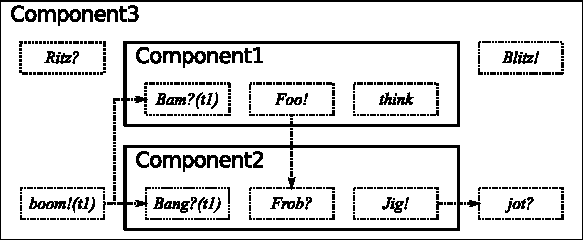
\includegraphics[width=\columnwidth]{system_model}
\caption{Example event detection system.}
\label{sys_model}
\end{figure}

As a mathematical abstraction the I/O automata model is appropriate for modeling reactive asynchronous and concurrent systems.
However, it lacks certain features needed to develop real components.
This subsection introduces these features and lays the foundation for adding the dynamics discussed in Section~\ref{dynamics}.

\paragraph*{Recursive Encapsulation}
Component frameworks that support recursive encapsulation allow components to contain other components.
Recursive encapsulation is at the heart of both bottom-up design strategies where smaller components are composed to produce larger ones, and top-down design strategies in which larger components are decomposed into smaller ones.
The contained component is the \emph{child} while the containing component is the \emph{parent}.
The resulting hierarchy helps developers organize programs by separating concerns and facilitates the reuse of existing components.
A distinction is made between the \emph{name} given to an instance and the \emph{type} of a child component to allow a parent component to contain multiple children of the same type.

Applying recursive encapsulation to I/O automata means that an I/O automaton may contain and use other I/O automata.
Recursive encapsulation implies that a parent automaton is the result of composing its children.
This definition excludes a parent from having any state or actions of its own.
Since it is often convenient to associate state and actions with a parent, we allow a parent to be the composition of its children and an anonymous child that contains the state and actions attributed to the parent.
The \emph{root automaton} is the automaton at the top of the hierarchy and represents the entire system as composition is applied recursively up the hierarchy.

Figure~\ref{sys_model} shows a sample event detector system where automata are depicted as solid rectangles.
The type of the automaton appears in a box in the upper left or lower left corner, e.g., Processor.
The name of a named automaton appears after its type, e.g., Converter C.
Actions are depicted as dotted rectangles and bindings are indicate by dotted lines with an arrow pointing to the input action.
Output actions are suffixed with \emph{!}, e.g., \emph{detect!}, input actions are suffixed with \emph{?}, e.g., \emph{detected?}, and internal actions have neither suffix, e.g., \emph{process1}.
The type associated with the value produced or consumed by an action is in parentheses after the name, e.g., \emph{out!(s)}.

The sample event detector system illustrated in Figure~\ref{sys_model} contains three automata (components):  an anonymous Processor, a Converter named C, and a Detector named D.
The Processor automaton is the root and C and D are its children.

\paragraph*{Explicit Composition}
Composition in the I/O automata model is based on actions having the same name and can be applied to an arbitrary number of automata.
Using recursive encapsulation, developers must have the ability to compose automata regardless of the naming convention used by the original developers.
To prepare for dynamic composition, we limit the scope of composition to associating a single output action with a single input action.
Such an association is called a \emph{binding} and consists of a pair $(output, input)$ where $output$ is the name of the output action and $input$ is the name of the input action.

Each automaton contains a set of bindings referring to its own actions, the actions of its children, the actions of its children's children, etc.
The automaton that prescribes a binding is said to \emph{own} that binding.
The global set of bindings can be used to rename input actions before applying composition as defined by the I/O automata model.
A map for renaming inputs is generated by replacing action names with their fully-qualified names in all bindings by tracing from the root automaton.
For example, the fully-qualified name of the $in?(s)$ action of the Converter C in Figure~\ref{sys_model} is $[root].C.in?(s)$.
Composition as defined by the I/O automata model can be applied after using the map to rename all input actions to their corresponding output action.
The map of bindings for the event detection system is 
\begin{displaymath}
\begin{split}
\{ ([root].out!(s), [root].C.in?(s)),\\
   ([root].C.out!(t), [root].D.in?(t)),\\
   ([root].D.detect!, [root].detected?) \}
\end{split}
\end{displaymath}

\paragraph*{Binding rules}
To be compliant with name-based composition under the I/O automata model, the set of bindings must adhere to certain rules.
First, the output action and input action of a binding must agree on the type being produced and consumed.
For example, an input action consuming an integer value can only be bound to an output action that produces an integer value.
The system shown in Figure~\ref{sys_model} follows this rule since $(out!(s), in?(s))$ agree on type $s$, $(out!(t), in?(t))$ agree on type $t$, and $(detect!, detected?)$ agree on the absence of a value (i.e., a signal).
Second, an input action can be bound to at most one output action.
Composing an input action with multiple output actions would introduce ambiguity into the relationship between the states of the automata and is therefore prohibited by the model.
A binding map where all bindings that mention the same input action are equivalent satisfies this rule.
For dynamics, which are discussed in Section~\ref{dynamics}, we must strengthen this rule to say that an input action can appear at most once in the global binding map.
This strengthened rule means that an input is the sink of at most one binding and that every binding has exactly one owner.
Third, an output action cannot be bound to more than one input action in the same automaton:  the state of the automaton containing the input actions would not be well-defined after the output is executed since the input action effects would be applied in an undefined order.
%% Let $\pi$ be a prefix operator that strips the action name (leaving the path and hence the automaton) of a fully-qualified action name.
%% The following must be true for the global binding map $B$:  $\langle \forall o : (o, z) \in B :: \langle \forall i,j : (o, i) \in B \land (o, j) \in B \land i \neq j:: \pi (i) \neq \pi (j) \rangle \rangle$.
Fourth, an output action cannot be bound to an input action in the same automaton.
Allowing such bindings would result in undefined behavior since the order of the output and input effects is undefined.
The I/O automata model prevents this by requiring that all actions belonging to the same automaton have a unique name.
To elaborate, we usually think about the output action occurring before the input action because a value must be generated.
However, the I/O automata model admits an interpretation where the value is generated first and the effects of the output action and input action are applied non-deterministically.
Graphically, an arrow originating in one component must terminate in another component, even if the latter is a child of the former as Figure~\ref{sys_model} illustrates.
%% To adhere to this rule, the following must be true for the global binding map $B$:  $\langle \forall o, i : (o, i) \in B :: \pi (o) \neq \pi (i) \rangle$.

\paragraph*{Concurrent execution}
Recall that composing I/O automata consists of concatenating state vectors and folding input actions into output actions and that the result of composition is a single equivalent automaton.
Since the state of each automaton is independent, opportunities exist for concurrent execution if the state of each automaton is preserved and a composition is not reduced to a single equivalent automaton.
Each local action implies a set of automata which in turn implies a set of state variables that might be modified.
For an internal action, this set consists of the automaton containing the internal action.
For an output action, this set consists of the automaton containing the output action and the automata that contain the input actions to which the output action is bound.
Two actions can be executed concurrently if their respective sets of state variables are disjoint.
The implied automata sets for each local action in Figure~\ref{sys_model} are: $out!(s) \to \{root, C\}$, $out!(t) \to \{C, D\}$, $process1 \to \{D\}$, $process2 \to \{D\}$, and $detect! \to \{D, root\}$.
Thus, $process1$ and $out!(s)$ can be executed concurrently while $process1$ and $detect!$ can not.

These observations create some interesting opportunities for designing and analyzing concurrent software.
Migrating intense computation to internal actions increases the level of parallelism in a system, i.e., the set of implied automata is small.
A high degree of fan-out (an output action being bound to many input actions) creates a bottle-neck and decreases the level of parallelism, i.e., the set of implied automata is large.
However, the input effects can be applied in parallel since the state of each automaton is independent.
A high degree of fan-in (an automaton has many bound input actions) also creates a bottle-neck by increasing the probability that two sets of implied automata will not be disjoint.
A scheduler might cluster and pin automata to processors to maximize concurrent execution while minimizing inter-processor communication.
Compositions of automata can be statically composed to take advantage of in-lining.
An individual automaton can be decomposed into a number of child automata to increase parallelism.

\paragraph*{Parameters and action types}
Actions in the I/O automata model can be defined using parameters.
Parameters are useful for situations requiring fan-in or session semantics.
For example, consider an automaton with an input action $in?(s)$ that is to be bound to $N$ different output actions.
To get around the limitation that an input can only be bound to one output, we augment the input action with a parameter that indicates the associated output action, e.g., $in?[i](s)$ where $i$ takes on the integer values from 1 to $N$.
\emph{Parameterized} actions take a parameter while \emph{unparameterized} actions do not.
Parameters, for actions that require them, are specified in the binding and serve to identify the action.

\emph{Unvalued} output and input actions produce and consume signals respectively.
\emph{Valued} output and input actions produce and consume values respectively.
The allowed combinations of input, output, and internal actions, unvalued and valued actions, and unparameterized and parameterized actions result in 10 possible action types:
unvalued unparameterized output (uv-up output),
unvalued parameterized output (uv-p output),
valued unparameterized output (v-up output),
valued parameterized output (v-p output),
unvalued unparameterized input (uv-up input),
unvalued parameterized input (uv-p input),
valued unparameterized input (v-up input),
valued parameterized input (v-p input),
unparameterized internal (up internal), and
parameterized internal (p internal).

\begin{figure}
\center
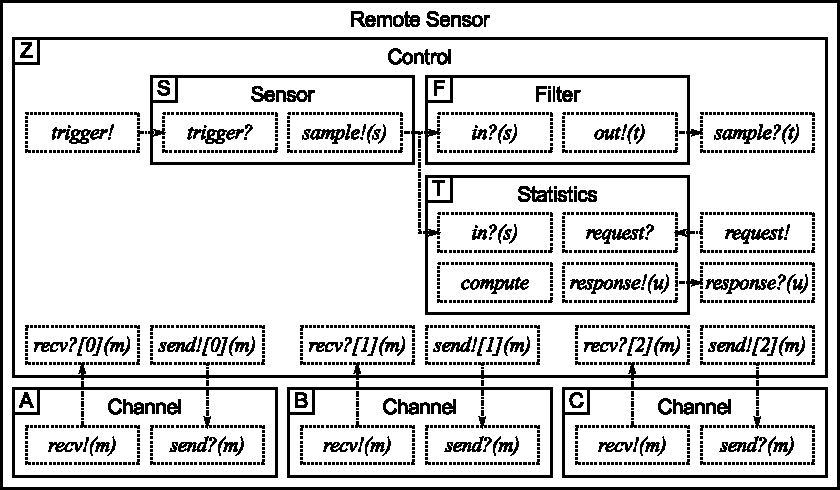
\includegraphics[width=\columnwidth]{example1}
\caption{Example remote sensor system.}
\label{example1}
\end{figure}

\paragraph*{Example}
Figure~\ref{example1} depicts a remote sensor system as a composition of automata using a scheme similar to Figure~\ref{sys_model} where parameters are given in brackets after the action name, e.g., \emph{recv?[0](m)}.
The Remote Sensor automaton consists of the Control automaton Z and three Channel automata A, B, and C representing three network connections.
The Control automaton Z consists of the Sensor automaton S, the Filter automaton F, and the Statistics automaton T.
The Control automaton C starts the sampling process with the uv-up output $Z.trigger!$.
The uv-up input $S.trigger?$ is executed atomically with $Z.trigger!$ due to the binding $(Z.trigger!, S.trigger?)$.
When the sampling process is complete, the v-up output $S.sample!(s)$ distributes the sample to the Filter F and Statistics component T via the $(S.sample!(s), F.in?(s))$ and $(S.sample!(s), T.in?(s))$ bindings.
Note that $S.sample!(s)$, $F.in?(s)$, and $T.in?(s)$ all agree on the type of the sample $s$.
The Filter automaton F passes the filtered sample to the Control automaton Z via the $(F.out!(t), Z.sample?(t))$ binding.
The Statistics automaton T calculates the statistics incrementally using the up internal $T.compute$.
The statistics can be polled by the Control automaton Z by issuing a request via the $(Z.request!, T.request?)$ binding and then receiving a response via the $(T.response!(u), Z.response?(u))$ binding.
The Control automaton Z contains a vp-output $Z.send![](m)$ and a vp-input $Z.recv?[](m)$ for sending and receiving network messages using the Channel automata A, B, and C.
The parameters 0, 1, and 2, are used to route messages to Channel automata A, B, and C respectively using the session idea mentioned previously.
Opportunities for concurrent execution exist for the remote sensor depicted in Figure~\ref{example1}.
The set of automata implied by $Z.trigger!$ is $\{Z, S\}$ while the set of automata implied by $T.compute$ is $\{T\}$.
Since the sets are disjoint, the two actions can be executed concurrently.

\subsection{Dynamics\label{dynamics}}

The I/O automata model assumes that systems are composed of a finite or countably infinite number of automata~\cite{lynch1996distributed}.
Assuming an countably infinite number of participants allows properties of the systems to be stated in terms of an abstract quantity representing the number of members, e.g., $N$, and is reasonable because all real systems are composed of a finite number of members.
The set of interactions in the I/O automata model is also fixed since automata are statically composed.
Dynamic systems are modeled by assuming that only a subset of the all the automata that could possibly exist are actively participating in the system.
To use this technique, a flag is associated with each automaton indicating if it is active or inactive and external actions for ``waking up'' and ``going to sleep'' are defined~\cite{lynch1996distributed}\footnote{Use the actual paper.  I think it has something to do with databases.}.

While assuming a fixed number of automata is reasonable for modeling, assuming a fixed number of automata for a real system results in over-provisioning or inflexibility.
To develop a component based on the static I/O automata model, a developer must choose a concrete value for the abstract quantity $N$.
System resources are wasted if the actual number of participants is much smaller than $N$.
If the number of participants is greater than $N$, then the system cannot respond to certain situations even though resources might be available.
Consequently, we add the ability to deal with a dynamic set of automata and interactions.

\paragraph*{System actions}
The four indivisible operations for managing a dynamic set of automata are \emph{create}, \emph{bind}, \emph{unbind}, and \emph{destroy}.
Create, bind, unbind, and destroy are collectively called \emph{system actions}.
The \emph{create} operation allows an automaton to create a child automaton.
The \emph{bind} operation allows an automaton to bind an input action to an output action while the \emph{unbind} operation allows an automaton to separate an input action from an output action.
The \emph{destroy} operation allows an automaton to recursively destroy a child automaton and all bindings associated with it.

System actions can fail for a variety of reasons.
A create fails if the automaton that should be added to the set of automata, i.e., the automata being created, already exists.
A bind fails if the automaton associated with the output action doesn't exist, the automaton associated with the input action doesn't exist, or any of the binding rules outlined in Section~\ref{practical} would be violated.
An unbind fails if the binding does not exist.
Note that the owner of binding is taken into account when determining if the binding exists so only the owner of a binding can dissolve it.
A destroy fails if the automaton being destroyed does not exist or is not a child of the automaton requesting the destroy action.

%% Let $A$ be the set of automata that exist where each element in $A$ is a pair $(p, a)$ where $p$ is the parent of $a$.
%% Let $B$ be the set of bindings that exist where each element in $B$ is a tuple $(w, o_a, o_n, o_p, i_a, i_n, i_p)$ where $w$ is the automaton that owns the binding, $o_a$ is the output automaton, $o_n$ is the name of the output action, $o_p$ is the parameter of the output action, $i_a$ is the input automaton, $i_n$ is the name of the input action, and $i_p$ is the parameter of the input action.
%% Define the predicate $exists (a) = \langle \exists p, q : (p, q) \in A :: q = a\rangle$ that is true when automaton $a$ exists, i.e., has a parent\footnote{The root automaton's parent is the special symbol $\perp$.}.
%% Define the predicate $existsb (a) = \langle \exists a : (w, o_a, o_n, o_p, i_a, i_n, i_p) \in B :: a = w \lor a = o_a \lor a = i_a \rangle$ that is true when automaton $a$ appears somewhere in $B$.
%% We define the create operation as the Hoare triple $\{exists (p) \land \lnot exists (a)\} \quad create(a)_p \quad \{(p,a) \in A\}$ which says that the parent automaton $p$ can create automaton $a$ if $p$ exists and $a$ does not exist.
%% The destroy operation can be defined $\{(p,a) \in A\} \quad destroy(a)_p \quad \{(p,a) \notin A \land \lnot existsb(a)\}$ which says that in order to destroy $a$ and remove all bindings associated with $a$, $p$ must be the parent of $a$.
%% Define the predicate $free (a, n, p) = \langle \forall w, o_a, o_n, o_p, i_a, i_n, i_p : (w, o_a, o_n, o_p, i_a, i_n, i_p) \in B :: \lnot (i_a = a \land i_n = n \land i_p = p) \rangle$ that is true when the input action argument is not bound.
%% Define the predicate $involved (o, n, p, i) = \langle \exists w, o_a, o_n, o_p, i_a, i_n, i_p : (w, o_a, o_n, o_p, i_a, i_n, i_p) \in B :: o_a = o \land o_n = n \land o_p = p \land i_a = i \rangle$ that is true when automaton $o$'s output action $(n, p, i)$ is bound to some input action in automaton $i$.
%% The bind operation can be defined $\{exists (w) \land exists (o_a) \land exists (i_a) \land free (i_a, i_n, i_p) \land \lnot involved(o_a, o_n, o_p, i_a) \land o_a \neq i_a \} \quad bind (w, o_a, o_n, o_p, i_a, i_n, i_p) \quad \{(w, o_a, o_n, o_p, i_a, i_n, i_p) \in B\}$ which says that in order for the binding to succeed the owner $w$ exists, automaton $o_a$ exists, automaton $i_a$ exists, the input action $(i_a, i_n, i_p)$ must not be bound, the output action $(o_n, o_p)$ of automaton $o_a$ cannot be bound to an input action in automaton $i_a$, and the automata $o_a$ and $i_a$ cannot be the same.
%% The precondition for $bind$ is same as the binding rules derived in section~\ref{system_model} augmented with existence tests for the owner, output automaton, and input automaton.
%% The unbind operation is similar to destroy: $\{(w, o_a, o_n, o_p, i_a, i_n, i_p) \in B\} \quad unbind (w, o_a, o_n, o_p, i_a, i_n, i_p) \quad \{(w, o_a, o_n, o_p, i_a, i_n, i_p) \notin B\}$.

% I didn't do more complex transactions, i.e., create-and-bind, because its not clear how it fails.
% Are partial successes allowed?
% Furthermore, such  transactions can be arbitrarily complex which doesn't bode well for efficiency.

\begin{figure}
\center
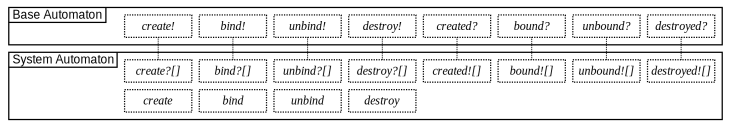
\includegraphics[width=\columnwidth]{system_action}
\caption{System actions.
  A base automaton contains output actions for creating, binding, unbinding, and destroying.
  The system automaton contains parameterized input actions for receiving the requests to create, binding, unbind, and destroy.
  The system automaton returns a result using the appropriate parameterized output action.
  The base automaton contains input actions to receive the results.}
\label{system_action}
\end{figure}

\paragraph*{The system automaton}
The set of automata $A$ and set of bindings $B$ are managed by the \emph{system automaton} which represents the run-time system.
Each automaton is composed (not bound) with the system automaton and has output actions for requesting system actions and input actions for receiving the results of system actions.
The system automaton, in turn, has input actions for receiving requests for system actions, internal actions for evaluating system action requests, and output actions for responding with the result of system actions.
Figure~\ref{system_action} shows the relationship between a base automaton and the system automaton.

Conceptually, the state variables $A$ and $B$ belong to the system automaton.
However, the state encoded by $A$ and $B$ is shared and used in the execution of every action.
The scheduler uses $A$ to ensure that only actions belonging to automata that exist are selected and uses $B$ to ensure that the appropriate set of input actions receive the value produced when an output action is executed.
Thus, the set of actions implied by any action is the set defined in Section~\ref{practical} \emph{and} and the system automaton.
However, the opportunities for concurrency explored in Section~\ref{practical} are not lost when one considers that the only actions that modify $A$ and $B$ must be serialized, i.e., not executed concurrently with other actions.

\paragraph*{Binding predicates}
The static configuration of a system as prescribed by the I/O automata model guarantees that the set of implied automata for an action is always the same.
This property is necessary and desirable for reasoning about the behavior of the system.
Admitting dynamics removes this guarantee since the set of implied automata will change according to the various system actions being executed.
To be specific, the set of implied automata for internal actions does not change but the set of implied automata for output actions can be changed with a successful bind, unbind, or destroy.

To force a dynamic system to behave like a static system, the execution of output actions must be delayed until the set of implied automata matches the set implied by the static system.
To do this, we take the conjunct of the precondition of an output action with a predicate over the set of bindings $B$ called a \emph{binding predicate} to ensure that the output action is not executed until its set of implied automata is correct.
Notice that this only requires reading $B$ and is permitted since all updates to $B$ are serialized as previously discussed.
Thus, a dynamic system can be analyzed as a static system by ignoring system actions and the binding predicates.
A static system can be implemented by adding binding predicates and logic to create the required constellation of automata.


\section{Design and Implementation\label{design}}

\begin{figure}
\center
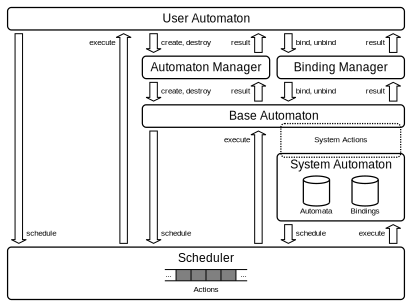
\includegraphics[width=\columnwidth]{architecture}
\caption{Framework architecture.}
\label{framework_architecture}
\end{figure}

The ioa++ framework is a C++ implementation of the component model described in Section~\ref{component_model} for POSIX environments .
The architecture of the ioa++ framework is depicted in Figure~\ref{framework_architecture}.

Conceptually, the set of automata $A$ and set of bindings $B$ belong to the system automaton.
However, the state they encode is shared and is used in the execution of every action.
A \emph{scheduler} uses $A$ to ensure that only actions belonging to automata that exist are selected and uses $B$ to ensure that the appropriate set of input actions receive the value produced when an output action is executed.
Thus, the set of actions implied by any action is the union of the set defined in Section~\ref{component_structure} and the system automaton.
The opportunities for concurrent execution discussed in Section~\ref{component_structure} hinge on the fact that \emph{only} actions that modify $A$ and $B$ must be serialized.
Binding predicates do not modify $B$ and therefore do not affect concurrent execution.
The scheduler is responsible for selecting and executing local actions subject to the I/O automata model and the concurrency constraints described in Section~\ref{component_model}.

All user automata inherit from a common base class (indicated by the Base Automaton layer shown in Figure~\ref{framework_architecture}) that provides facilities for asynchronously creating and destroying child automata and bindings.
The Base Automaton layer provides statically composed system actions that are used to communicate with the system automaton.
In most situations, the services provided by the Base Automaton layer are too low-level to be used directly by a user automaton.
Instead, an Automaton Manager provides a common higher-level interface for asynchronously managing a single child automaton using the services of the Base Automaton layer.
Similarly, a Binding Manager presents a high-level interface for asynchronously managing a single binding.

\subsection{Scheduler\label{scheduling}}

The scheduler is responsible for both selecting and executing local actions.
These two activities are decomposed into a \emph{dispatcher} that executes actions and a \emph{controller} that selects the next action.

The dispatcher enforces the execution and concurrency constraints of Section~\ref{component_model}.
Input actions are executed with corresponding output actions, according to the current set of bindings.
The dispatcher allows actions to be executed concurrently by (1)~requiring that the sets of automata implied by each action are disjoint and (2)~serializing all updates to the set of automata and bindings.

Since concurrent access to the dispatcher is allowed, the dispatcher implementation the dispatcher must be thread-safe.
Our implementation of the dispatcher uses a two-level locking scheme to enforce the concurrent execution constraints.
Any action that modifies the set of automata and bindings must first acquire a write lock to prevent concurrent access.
All other actions acquire a read lock to implement single-writer/multiple-reader semantics.
The second phase of executing a non-modifying action involves acquiring locks for the set of automata implied by an action.
The locks are acquired in a fixed order to prevent deadlock~\cite{havender1968avoiding}.
Once the locks are acquired, the precondition is evaluated, the local action and all bound input actions are executed, and the locks are released.

The controller encodes a \emph{policy} that selects the next local action.
For the framework to be a valid implementation of the I/O automata model, the controller used by the scheduler must be \emph{fair} as defined in Section~\ref{component_model}.
The run-time system can be initialized with different controllers to achieve different performance objectives.
To leverage the power of different operating system mechanisms without exposing users to their complexities directly, the ioa++ framework is designed so that all native concurrency and synchronization mechanisms (e.g., threads and mutexes) are encapsulated within the dispatcher and controller.
For example, a controller can be written to use multiple threads of execution to exploit fully the concurrency inherently available in a system of automata,
while still providing concurrency semantics in a manner consistent with the I/O automata component model.

\paragraph*{Explicit dynamic scheduling}
The I/O automata model assumes that the scheduler knows about every local action in the system.
There are two approaches for achieving this in practice.
In the first approach, automata declare \emph{statically} all of their actions to the scheduler.
The controller then has the responsibility of cycling through the actions according to some fair policy.
Since the scheduler has no knowledge about which actions are \emph{enabled} or \emph{disabled} (have a precondition that is true or false respectively), this approach reduces to naively trying each action.

A more focused approach, which is the approach used in our framework implementation, is to allow automata to declare \emph{dynamically} the actions they would like the scheduler to consider.
%The act of declaring an action to the scheduler is called \emph{scheduling}.
The controller then has the responsibility of processing the set of requested actions according to some fair policy.
Observe that executing an action potentially changes the state of the automaton and causes the set of enabled actions to change.
Consequently, an automaton is given the opportunity to declare actions to the scheduler (i.e., to \emph{schedule} them) after one of its actions is executed.
Since the state variables (and therefore preconditions) of all automata are independent, each automaton is responsible for scheduling its own actions.
For bootstrapping, each automaton is allowed to schedule actions when it is created.

In this approach, scheduling disabled actions is unnecessary.
In order for a scheduled disabled action $a$ to become enabled, the automaton associated with the action must change state by executing another enabled action $b$ sometime after $a$ is scheduled.
Consequently, the scheduling of the disabled action $a$ can be deferred until the execution of some other action.
Notice that refraining from scheduling disabled actions does not affect the fairness of the scheduler since they cannot cause a state change when selected.
This result leads to a guarded programming idiom where the precondition of each action is checked before it is added to the schedule.

However, an automaton must still ensure that the scheduler will \emph{consider} all actions that are currently enabled.
A simple technique for accomplishing this is to schedule all enabled actions.
More efficient schemes are possible if one considers how an action might enable other actions and which actions have already been scheduled.
However, this must be done carefully, since not considering an enabled action would violate the fairness of the controller.
% since it will never select an action that may cause a state change.
% Not scheduling an (enabled) action is a common mistake.

\paragraph*{Binding predicates and scheduling}
%% This assumption is not implicit because we state that the preconditions are independent.
The preceding discussion on scheduling assumed that an action in one automaton cannot affect preconditions in another automaton.
This is not entirely correct when one considers the system automaton and binding predicates.
For example, imagine an automaton with a single output action whose only precondition is that it must be bound and assume that the automaton only schedules the action when enabled.
When the automaton is created, its only action is disabled.
Consequently, it will not schedule its action and therefore will not be executed.
Suppose that some time after the automaton is created, another automaton successfully binds to the output action.
The bind action changes the precondition but the automaton will never be executed since it has no way of scheduling the output action.
While this example may seem contrived, it is representative of situations where an automaton is waiting for one or more of its outputs to be bound: a situation that occurs quite often in practice.
To remedy this, our framework takes advantage of the fair scheduling criteria of the I/O automata model and schedules an output action after each successful bind or unbind.

\paragraph*{Actions of no-longer-existing automata}
Every action in the set of actions considered by the controller is scheduled by its associated automaton.
Since automata can be destroyed, an action in the set owned by the controller might belong to an automaton that no longer exists.
Our solution is to check if the automaton exists before executing an action.
This check is performed by the dispatcher and avoids the overhead associated with synchronizing the set of actions with the set of automata every time an automaton is destroyed.
Our solution assigns each automaton a unique identifier assuming that the set of automata in the system turn over less frequently overall than the set of actions that have been scheduled.

\paragraph*{Delayed actions}
Scheduling activities for a future time is a useful feature for many systems because it allows the system to sleep between activities. For example, the framework should support the development of automata that act as timers and alarms.
Conceptually, an action is held until the time associated with it, at which point it is added to the set of actions being considered by the scheduler.
Actions scheduled in the past or present are released immediately to the scheduler.
When the same action is scheduled at two different times, the earliest time is used.
% Things I didn't say:  No canceling.

\paragraph*{File descriptor events}
File descriptors are used to communicate with the outside world in a POSIX environment.
Observe that there is no concept of blocking in the I/O automata model and introducing blocking I/O operations into action effects may adversely affect the asynchronous and concurrent nature of I/O automata.
Thus, we require techniques that allow a program (1) to wait until a file descriptor is asynchronously ready for I/O and (2) to perform non-blocking I/O operations.
This implies the use of either the Proactor or Reactor pattern~\cite{schmidt2000pattern}.
The ioa++ framework uses the Reactor pattern since (1) it is simpler and (2) many operating systems have non-blocking I/O and some kind of synchronous I/O (de)multiplexing, whereas asynchronous I/O is less widespread.

Our use of the Reactor pattern causes an action to be scheduled when a file descriptor is ready for reading or writing.
A user automaton creates a file descriptor and configures it for non-blocking I/O.
The automaton then tells the scheduler to release an action (typically an internal action) whenever the automaton becomes ready for reading (or writing).
Subsequent requests made using the same file descriptor and event (ready for reading, ready for writing) are ignored.
Once the file descriptor is ready, the action is released for consideration by the controller.
The scheduler also provides a special function for closing file descriptors that purges them from the reactor.

\paragraph*{Basic and multi-threaded schedulers}
The ioa++ framework distribution provides both a basic scheduler that is single-threaded and uses a single queue of actions that is processed using first-in/first-out semantics, and a multi-threaded scheduler with a configurable number of threads that we use in the performance evaluation described in Section~\ref{evaluation}.
Scheduling is idempotent to prevent unbounded growth of the queue, and both scheduler implementations use the Reactor pattern to implement delayed actions and file descriptor events.

\subsection{System Actions\label{system_action_section}}

Our approach to system actions follows the model introduced in Section~\ref{dynamics}.
All automata are statically composed with a system automaton via system actions for dynamically creating child automata, binding external actions, unbinding external actions, and destroying child automata.
The system automaton implements a request-response protocol where an automaton requests a system action and the system automaton processes the request and responds with an indication of either success or failure.
Associated with each request is a \emph{subject} which is the automaton's local name for an automaton or binding.
Subjects allow an automaton to have multiple requests outstanding at once.

Automata use a simple protocol for creating and destroying child automata.
Each child automaton is represented by a unique subject which is in one or two of five states: CreateSend, CreateRecv, CreateDone, DestroySend, and DestroyRecv.
Subjects start in the CreateSend state which indicates that the request for this subject is waiting to be sent to the system automaton.
Once the request has been sent, the subject transitions to the CreateRecv state and waits for a response from the system automaton.
Once the system automaton sends the response, the subject transitions to the CreateDone state.
When the user automaton requests that the child automaton be destroyed, the subject is either (1) added to the DestroySend state if the subject is in CreateRecv or CreateDone or (2) removed from all states if the subject is in CreateSend.
A subject appearing in both CreateDone and DestroySend transitions to the DestroyRecv state when the automaton makes the request to destroy it.
The system automaton can process system actions in any order.
This protocol ensures that an automaton doesn't request that a child automaton be destroyed until it receives confirmation that it was created.
The subject is forgotten when the system automaton responds with the result of the destroy action.

The protocol for binding is similar but addresses the possibility that a binding can be dissolved at any point due to the asynchronous destruction of automata.
We define analogous states for the binding state machine: BindSend, BindRecv, BindDone, UnbindSend, and UnbindRecv.
A binding subject can be in either BindRecv, BindDone, UnbindSend, or UnbindRecv when it receives a result from the system automaton indicating that the binding was dissolved.

\paragraph*{Automaton and Binding managers}
The protocol used by automata to asynchronously manage child automata and bindings is suitable for simple constellations but becomes unwieldy when creating more complicated ones.
Automaton Managers and Binding Managers provide individualized facades to the system action state machines.
Creating an Automaton Manager initiates the creation of a new child automaton and invoking a destroy method initiates the destruction of a child automaton.
Automaton Managers can be monitored using the Observer~\cite{gamma1995design} pattern to determine when and how the creation/destruction process succeeds.
Binding Managers are similar except they do not begin the process of binding until the automata providing the output action and input action have been created: thus, Binding Managers observe Automaton Managers.

\ifjournal
\paragraph*{Generators}
A \emph{generator} is a single-use factory for creating an instance of an automaton.
Generators are used to produce new automata as part of the create system action and are visible as arguments in the various layers of the framework.
\fi


\section{I/O Automata Representation and Programming Model\label{representation}}

In this section, we show how I/O automata are represented using our framework and how they can be used to construct programs.
We develop a simulation for a distributed algorithm to show the basic features of the framework and then show a real implementation of the same algorithm.
The problem we consider is that of electing a leader in unidirectional ring.

The algorithm we consider is the asynchronous LCR algorithm presented by Lynch in Chapter 15 of~\cite{lynch1996distributed} which is in turn based on the work of LeLann~\cite{} and Chang and Roberts~\cite{}.
The LCR algorithm assumes that every node has a unique identifier.
Each node begins by assuming that it is the leader and send its own unique id to its neighbor.
If a node receives a unique id from its predecessor that is greater that the id that it believes to be the leader, then it changes its belief about the leader to the new id and sends the new id to its successor.
When a node receives its own id, it elects itself the leader of the ring.

\subsection{The AsynchLCR Automaton}

Appendix~\ref{asynch_lcr} shows the code for the asynchronous LCR automaton.

All automaton inherit from the \verb+ioa::automaton+ base class which implements the system call interface expected by the system automaton.
The \verb+asynch_lcr_automaton+ inherits from the \verb+ioa::automaton+ base class (line 13-14).

The state variables of the automaton are captured as members variables.
The \verb+m_u+ variable stores the id of node that this id believes to be the leader (line 23).
The \verb+m_send+ variable is a queue that stores ids that will be sent to the next node in the ring (line 24).
The \verb+m+status+ variable is used by the leader to report its election (line 25).

The constructor allows for initialization of the state variables and bootstrapping the scheduler.
The unique id of the automaton is a random number with ties broken by the index of the automaton.
Every node assumes that they are the leader initially \verb+i+ (line 29).
All nodes start in the unknown state (line 30).
Each node starts by sending their id to their neighbor (line 32).
The automaton bootstraps the scheduler after its state variable are initialized (line 33).

Actions consist of member variables that implement the Action concept.
An easiest way to declare these variables is to use a macro for the appropriate action type.
The \verb+asynch_lcr_automaton+ contains a \verb+send+ output action (line 53), a \verb+receive+ input action (line 73), and a \verb+leader+ output action (line 90).
The macros assume that actions are encoded using two or three functions.
Local actions require a precondition named \verb+action_name_precondition+ that returns true if the action is enabled (line 37, 76).
Notice that the preconditions are declared \verb+const+ since they should not change the state of the automaton.
All actions require an effect named \verb+action_name_effect+ that encodes the effect of the action (line 42, 56, 81).
All actions also require a scheduling function named \verb+action_name_schedule+ that allows the automaton to schedule actions (line 48, 68, 85).
Notice that the schedule functions are also declare \verb+const+ for the same reason as the preconditions.

In the I/O automata model, the send precondition only requires that the send queue not be empty (line 38).
However, if the send action executes before it is bound, the id at the front of the send queue will be lost.
Consequently, we add a binding predicate that ensures that send output is bound to at least one input (line 39).
The \verb+ioa::binding_count+ function returns the number of actions bound to the given action.
This is non-negative for output actions, 0 or 1 for input actions, and 0 for internal actions.

The send action is a valued unparameterized (v-up) output.
The value produced by send has the type \verb+UID_t+ (line 42).
Notice that this agrees with the type in the action declaration (line 53).
Similarly, the receive action is a valued unparameterized (v-up) input action that accepts a value of type \verb+UID_t+ (line 56, 73).
Notice that input action effects take a constant reference.

The send action removes and returns the id at the front of the queue (line 42-46).
The receive action updates the current leader sending it to nodes successor and confirms an election (line 56-66).
Once a node is chosen as the leader, it reports it using the leader action (line 81-83).

After every action is executed, the associated scheduling function is called.
All scheduling calls in the \verb+asynch_lcr_automaton+ dispatch to the same member function (line 93-100).
The \verb+asynch_lcr_automaton+ uses the strategy outlined in section~\ref{design} and checks the precondition of each action before scheduling it.

\subsection{AsynchLCR Simulation}

For a simulation of the AsynchLCR algorithm, we connect each node using a channel automaton.
The channel automaton is introduced by Lynch in Chapter 8 of ~\cite{lynch1996distributed} and listed in appendix~\ref{channel}.
The channel automaton takes a template parameter for the messages transported by the channel.

Appendix~\ref{ring} contains an automaton that creates the ring.
The template parameter \verb+T+ represents the automaton, i.e., \verb+asynch_lcr_automaton+, and the template parameter \verb+M+ represents the message type for the channel automata, i.e., \verb+UID_t+.
The size of the ring to simulate is passed as the constructor argument \verb+N+ (line 9).

The constructor for the ring starts by declaring vectors to hold automaton managers for the LCR automata (line 12) and automaton managers for the channels (line 13).
The loop in (line 15-20) initializes the vectors.
The \verb+ioa::make_automaton_manager+ function creates automaton managers.
These require action to an \verb+ioa::automaton+ which is always provided by a \verb+this+ pointer and a generator as described in section~\ref{design}.
The \verb+ioa::make_generator+ creates a generator.
Generators take constructor arguments for the automaton they will produce and pass them to the constructor when the automaton is allocated.
For example, the LCR automata are initialized with an index (line 17).

The loop in (line 22-33) creates the various bindings necessary to create the ring and receive the leader election.
The \verb+ioa::make_binding_manager+ function creates binding managers.
This function requires access to an \verb+ioa::automaton+ to realize the system actions.
The other arguments are the automaton managers and actions for the output action and input action.
For example, the send action of the LCR automaton is bound to the send action of the successor channel in (line 23-25).
Similarly, the receive action of the LCR automaton is bound to the receive action of the predecessor channel in (line 26-28).

The ring automaton contains a single unvalued parameterized (uv-p) input action for receiving the leader (line 36-38).
The parameter \verb+i+ is the index of the LCR automaton.
The leader actions are bound in (line 29-31).
Notice that the parameter for the leader input action is set in the call to \verb+ioa::make_binding_manager+.

Binding to an automaton that already exists requires an object that behaves like an automaton manager but refers to an automaton that already exists.
Objects of the \verb+ioa::handle_manager+ class satisfy this requirement.
The ring automaton declares a handler manager \verb+m_self+ (line 6) and initializes it with its automaton identifier (line 10).
Associated with each automaton is a unique identifier called an \emph{aid} which can be retrieved with \verb+ioa::get_aid+.

Appendix~\ref{driver} contains the driver program for the LCR simulation.
A global FIFO scheduler \verb+sched+ is declared on (line 11).
The scheduler is started with the \verb+ioa::run+ function (line 12).
The \verb+ioa::run+ function starts the scheduler using the root automaton returned by the specified generator which in this case is the ring automaton.

\subsection{AsynchLCR Implementation}

%% Conclude with our recommendations for programming, highlight need for exploration.

%% Tips for Writing Programs with I/O Automata
%% 1. Make sure that a parameter exists.
%% 2. Move logic in observe to local actions.
%% 3. Avoid observing an arbitrary number of managers.
%% 4. Do not bind to managers allocated on the stack.
%% 5. Stop when an error is encoutered and report it.
%% 6. Make sure output actions are bound.
%% 7. Make sure local actions are scheduled.
%% 8. Do not pass pointers---use const_shared_ptr.
%% 9. Check preconditions.
%% 10. Check effects.
%% 11. Order clauses of preconditions for efficiency.
%% 12. Automata that should be destroyed at the same time should be created at the same time and vice versa.  (Group using a parent.)

%% \begin{outline}
%% \item State
%%   \begin{outline}
%%   \item There is no shared state in a 
%%   \item Local state only
%%   \item Shared state
%%     \begin{outline}
%%       \item Impossible in distributed systems
%%       \item Dangerous in local systems
%%     \end{outline}
%%   \end{outline}
%% \item Communication
%%   \begin{outline}
%%   \item Atomic asynchronous message passing
%%   \item Network sets size of atom (UDP)
%%   \item Can build reliable streams (TCP)
%%   \item Local equivalent is passing a value
%%   \item Model should lend itself to writing protocols
%%   \end{outline}
%% \item Asynchrony
%%   \begin{outline}
%%     \item Model must have natural support for asynchrony, i.e., event-based
%%     \item Leads to a more efficient implementation because changed state and enabled actions become obvious
%%   \end{outline}
%% \item Concurrency
%%   \begin{outline}
%%     \item Reason about systems using non-deterministic interleaving of atomic actions
%%     \item Model should admit implementations that execute concurrently
%%   \end{outline}
%% \item Dynamics
%%   \begin{outline}
%%     \item Configuration - Edges in graph of communicating components can change at run-time.
%%       \begin{outline}
%%       \item Already required in distributed settings
%%       \item Not addressed in formal models
%%       \end{outline}
%%     \item Extension - Nodes in graph of communicating components can change at run-time.
%%   \end{outline}
%%   \item Reflection
%% \end{outline}

%% I/O Automata
%% \begin{itemize}
%%   \item Compare with UNITY
%%   \item Compare with esterel
%%   \item Compare with pi calculus
%%   \item Compare with Ptolemy
%% \end{itemize}


\section{Evaluation\label{evaluation}}

The ioa++ framework permits independent actions to be executed concurrently.
The goal of this evaluation is to show that the degree of exploitable concurrency depends only on (1) the interactions of the I/O automata comprising a system, and (2) the overhead of the framework which this evaluation serves to quantify for our current implementation of ioa++.

To evaluate concurrent execution, we examine a system whose actions can be configured to span the range from having no independent actions to having only independent actions.
We measure the time required to execute a fixed number of actions using a scheduler with a configurable number of threads.
We then calculate the speed-up by comparing an execution using one thread to an equivalent execution using two threads.
We also vary the complexity of each action to gain insight into how overhead and synchronization affect concurrent execution.

An automaton of type $R$ contains an input, output, and internal action.
The output and internal action effects execute an algorithm whose complexity is proportional to the parameter $N$.
The automaton executes a fixed number of local actions.
The automaton schedules the internal action with probability $\sqrt{\rho}$ and schedules the output action otherwise.
The system $S$ to be executed consists of two $R$ automata composed so the output action of one is composed with the input action of the other.
If we divide the execution into rounds where each automaton executes a single action, the probability that both $R$ automata execute an internal action is $\sqrt{\rho} \times \sqrt{\rho} = \rho$.
Thus, we can use the parameter $\rho$ to vary the independence of the automata.

For this experiment, we used a simple multi-threaded scheduler that assigns each local action to a thread based on the automaton identifier of the local action using the techniques described in Section~\ref{scheduling}.
When the scheduler is configured to use a single thread, all actions are executed by that same thread.
When two threads are used, one thread executes the actions of one $R$ automaton while the other thread executes the actions of the other $R$ automaton.

A trial consists of a choice for $\rho$, $N$, and the number of actions to be executed.
For our experiments, the parameter $\rho$ was varied from $0.0$ to $1.0$ in increments of $0.1$ and the parameter $N$ was varied from $1$ to $1000000$ by factors of $10$.
The number of actions executed by each automaton was fixed at 1000.
Each trial was repeated 1000 times.
All calculations were performed assuming a normal distribution at a confidence level of 95\%.

The driver for a single trial can be found in examples/random.cpp\footnote{\url{github.com/jrwilson/ioa/blob/master/examples/random.cpp}} of the ioa++ package.
The trials were performed on a Mac G4 running OS X 10.5.8 with two 2.66 GHz Dual-Core Intel Xeon processors with 2GB of memory.
The code was compiled and linked with i686-apple-darwin9-g++-4.0.1 build 5493 with -O2 optimization and the -DPROFILE flag to enable profiling in ioa++.

\begin{figure}
\center
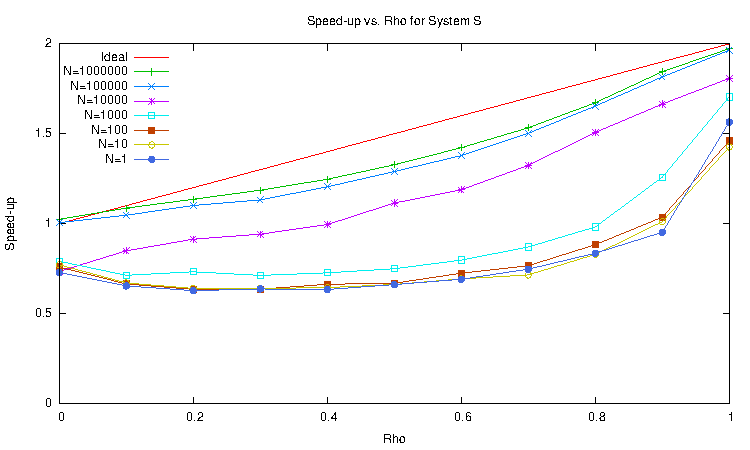
\includegraphics[width=\columnwidth]{speed_up}
\caption{Speed-up for system $S$.\label{speed_up}}
\end{figure}

Figure~\ref{speed_up} shows the speed-up when system $S$ was executed with two threads versus one thread.
Confidence intervals are shown but are negligible with the largest being a speed-up range of $\pm$0.0165.
When $\rho = 0$, every action is a bound output action and therefore depends on both $R$ automata.
Consequently, every action must be serialized yielding a maximum speed-up of 1.
When $\rho = 1$, every action is an internal action and can be executed concurrently with a corresponding maximum speed-up of 2.

The speed-up shows a strong dependence on the duration of each local action which is proportional to $N$.
A small value for $N$ means that very little time is spent executing automaton code.
Consequently, a greater fraction of time is spent executing framework code which includes various synchronization calls to the pthreads library.
For a small enough $N$, this overhead dominates the execution time.
This situation is exacerbated by multiple threads since they will actively interfere with one another which can be seen in the slow-down for small values of $N$.
Conversely, when $N$ is large, relatively little time is spent executing framework and synchronization code.
Consequently, contention is reduced allowing for greater speed-ups as indicated by Figure~\ref{speed_up}.

\begin{figure}
\center
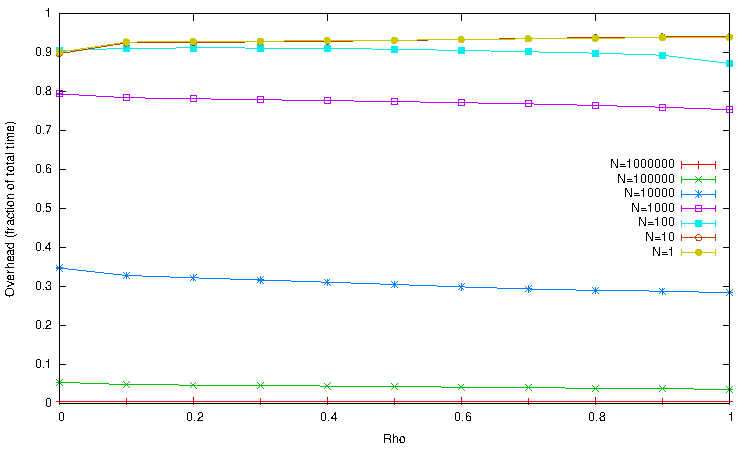
\includegraphics[width=\columnwidth]{overhead1}
\caption{Overhead for system $S$ when using one thread.\label{overhead1}}
\end{figure}

\begin{figure}
\center
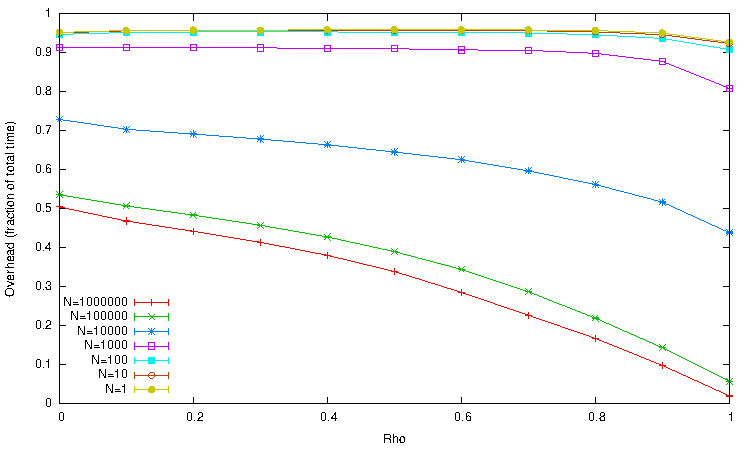
\includegraphics[width=\columnwidth]{overhead2}
\caption{Overhead for system $S$ when using two threads.\label{overhead2}}
\end{figure}

Figures~\ref{overhead1} and \ref{overhead2} show the average per thread of the fraction of time devoted to framework code and synchronization calls for the single and multi-threaded executions; confidence intervals are again negligible with largest being $\pm$0.002155 for Figure~\ref{overhead1} and $\pm$0.001781 for Figure~\ref{overhead2}.
Since the number of actions to be executed is constant, the single threaded execution shows a relatively consistent fraction for each value of $N$.
The fraction decreases as $\rho$ goes to 1 and the system transitions from acquiring two locks to one lock.
The multi-threaded execution shows that the fraction of time devoted to system overhead decreases as $\rho$ goes to 1 and is more pronounced when $N$ is large.
For example, when $N=1000000$ one thread spends half of its time waiting on the other thread when $\rho = 0$ and spends very little time on synchronization when $\rho = 1$.

This experiment indicates that although concurrent execution is possible with ioa++, a significant speed-up will only be achieved if (1) enough independent actions are enabled and (2) the durations of the independent actions are large relative to the overhead of ioa++.
The overhead of ioa++ can be divided into three components corresponding to the time it takes to dispatch an action, the time required to synchronize using the pthreads library, and the time required to add an action to the scheduler via the ioa::schedule call.
From the results, we calculated the average overhead per action of the ioa++ framework when dispatching an action and found it to be 4316ns $\pm$ 3.5ns for the single threaded experiments and 6067ns $\pm$ 3.6ns for the multi-threaded experiments.
Similarly, we calculated the scheduling overhead and found it to be 247ns $\pm$ 0.678ns for the single threaded experiments and 307ns $\pm$ 0.357ns for the multi-threaded experiments.
Both of these potentially can be improved with better scheduler design.
The synchronization time depends on the interactions among the automata comprising the system, the scheduler, and the locking scheme used by the framework.
We plan to optimize scheduling and synchronization performance in ioa++ as future work.


\section{Related Work\label{related_work}}

Our development of ioa++ grew out of the challenges faced when trying to develop distributed systems with threads.
Lee elaborates on the problems faced when using threads for concurrency in~\cite{lee2006problem}.
Given the shift from higher clock frequencies to larger numbers of cores as the driver of hardware performance, these same concerns are relevant to trends that look to deliver performance improvements through increasingly concurrent programs~\cite{sutter2005software}.

Leveraging a formal model of concurrency to make concurrent programming easier is a well established technique.
We consider three exemplars that are most relevant to the discussion in this paper: Communicating Sequential Processes, Actors, and I/O automata.
Of these, we selected the I/O automata model of Lynch and Tuttle\cite{lynch1987hierarchical} because of its support for features essential to developing distributed systems~\cite{lynch1996distributed}.
%% Temporal logic proof techniques~\cite{manna1992temporal},~\cite{lamport1978time} also can be used to reason about I/O automata, towards developing \emph{correct} systems.

The Communicating Sequential Processes (CSP) model~\cite{hoare1978communicating} is a popular technique for modeling concurrent systems.
The fundamental concurrency control primitive in CSP is the \emph{rendezvous} which allows processes to synchronize and possibly exchange values.
CSP was influential in the design of the occam programming language~\cite{jones1987programming} and continues to influence the design of modern programming languages, e.g., Go~\cite{go}.

An actor~\cite{agha1986actors} is a behavior that can perform a number of actions when receiving a message including (1) replacing itself with a new behavior, (2) sending messages to other actors, and (3) creating new actors.
The Actor model has influenced the design of languages such as Erlang~\cite{armstrong1996concurrent} and Scala~\cite{odersky2004overview}.

% The direct implementation of a formal model to simplify concurrent programming was inspired by the application of structured programming~\cite{dijkstra1968letters} to programming language design.
% Structured programming simplifies development by allowing programmers to reason about their programs directly from the source code; regardless of whether of not the code is formally verified.
% The collective formalization of threads, i.e., semaphores~\cite{dijkstra1968cooperating}, monitors~\cite{hoare1974monitors}, etc., appears in popular libraries, e.g., POSIX threads~\cite{butenhof1997programming}, and languages, e.g., Java~\cite{christopher2000high}.

%% Frameworks for reusable asynchronous and concurrent modules
%%   Collective formalization of threads
%%     CORBA (asynchronous method invocation)/RMI/RPC (function call stack model, ~threads)
%%   CSP
%%   Actors

%% Comparing I/O automata to every model for asynchronous, concurrent, and distributed computing is beyond the scope of this paper, so we focus instead on exemplars.
%% The I/O automata model is based on state transitions which matches the imperative style that dominates modern concurrent programming.
%% This is similar to the motivation for UNITY~\cite{chandy1988parallel} and is in contrast to functional models such as the $\pi$-calculus~\cite{milner1992calculus} and actors~\cite{agha1986actors}.
%% The I/O automata model assumes independent state with explicit communication, like communicating sequential processes (CSP)~\cite{hoare1978communicating} but unlike threads~\cite{lee2006problem} or the UNITY model~\cite{chandy1988parallel}.

%% All models for asynchronous, concurrent, and distributed computing admit non-determinism.
%% Lee points out that the difficulties of thread-based programming come from a need to ``prune'' non-determinism when paired with shared state and adopts the view that software components should be deterministic with respect to concurrency save a few that introduce non-determinism in a controlled way~\cite{lee2006problem}.
%% Programs in UNITY are composed by concatenating program texts and resolving shared variables~\cite{chandy1988parallel}.
%% For this reason, they share many of the same concerns as threads under composition.
%% I/O automata can be viewed as taking an alternate approach by admitting non-determinism while prohibiting shared state.
%% In I/O automata, the sequential flow control seen with threads~\cite{lee2006problem} and CSP~\cite{hoare1978communicating} is replaced by the non-deterministic execution of conditional atomic actions which resembles execution in the UNITY model~\cite{chandy1988parallel}.
%% The ability to create new automata can be compared to actor creation in the actor model~\cite{agha1986actors}.
%% Actors communicate by name using a buffered mail system while communications in I/O automata are not buffered and anonymous.

% Other efforts to implement I/O automata have focused on simulation and verification~\cite{goldman1990distributed},~\cite{georgiou2009automated}.
% As observed in~\cite{georgiou2009automated}, a benefit of implementing distributed systems directly with I/O automata is the ability to reason about the behavior of a system or component directly from the source code using techniques from the I/O automata formalism.
% However, where~\cite{georgiou2009automated} introduces a new language and uses the Message Passing Interface (MPI)~\cite{gropp1999using} library for communication, ioa++ uses the existing C++ language and exposes native operating system services.

To our knowledge, the Spectrum Simulation System~\cite{goldman1990distributed} and the IOA language~\cite{garland2003ioa} are the only existing approaches that allow one to execute a system expressed as a collection of I/O automata.
Spectrum focuses on algorithm development through simulation.
IOA focuses on formal software development including both simulation and verification.

The ioa++ framework can be compared directly to the IOA language due to the availability of a compiler~\cite{tsai2002code},~\cite{tauber2004verifiable},~\cite{tauber2004compiling} that has been used to implement a number of protocols~\cite{georgiou2009automated}.
\cite{georgiou2009automated} lists six challenges when developing the compiler: ``Program structuring,'' ``IOA Programs and external services,'' ``Modeling procedure calls,'' ``Composing automata,'' ``Nondeterminism'', and ``Implementing datatypes.''
Programs written in IOA are compiled into Java and executed on hosts communicating using the MPI library.
IOA requires programs to be presented in a ``node-channel'' form that allows them to be composed with built in ``mediators'' that implement external services such as MPI.
IOA lacks support for procedure calls, which complicates modeling and interfacing with external services, especially when a procedure call may block.
The IOA compiler composes automata statically using a ``composer'' resulting in a ``node automaton.''
The next action to be executed is selected by a function that resolves the non-determinism in the schedule.

IOA and ioa++ represent two fundamentally different approaches to programming directly with I/O automata.
The development of a new language was necessary for IOA due to its focus on formal verification.
% On the other hand ioa++ uses the existing C++ language and compilers.
IOA encapsulates external services using built in ``mediators'' while ioa++ exposes operating system services via file descriptors, relying on the programmer to ensure non-blocking operation.
IOA focuses on static composition to produce a single node program while ioa++ focuses on dynamic composition and allows concurrent execution.
Both IOA and ioa++ require the programmer to add code to schedule actions, which may be a common source of errors.
In IOA, the programmer provides a deterministic scheduling policy.
Scheduling in ioa++, however, is non-deterministic according to the global policy encoded by the controller.

%% CORBA thread model

%% %% Lee~\cite{lee2006problem} also identifies a number of strategies for coping with thread-based programming including libraries, patterns, programming languages, and coordination languages.
%% %% In~\cite{schmitd2000patterns}, Schmidt et al. describe patterns for developing asynchronous and concurrent objects and systems.
%% %% The Split-C~\cite{culler1993parallel} and Cilk~\cite{blumofe1995cilk} add features to the C programming language for multi-threaded computation.
%% %% The Erlang~\cite{armstrong1996concurrent} 

%% Ada

%% The 

%% Events

%% Lynch

%% Garland

%% Ken Goldman

%% proactor/reactor
%% Observer



\section{Conclusion and Future Work\label{conclusion}}

I/O automata are a good foundation for asynchronous and concurrent components due to independent state, well-defined interfaces, and well-defined interactions under composition.
The ioa++ framework facilitates concurrent execution via dynamic composition and the degree of concurrency is limited by the interactions of the automata and the overhead of the framework.
The two key challenges when moving from the formal model to an actual implementation were introducing features for managing dynamic constellations of automata and providing a concrete scheduling mechanism.
We believe that attempts to implement other formal models, e.g., UNITY, will have similar experiences and thus encounter the differences between theory and practice.
We agree with~\cite{georgiou2009automated} that having a representation of a model that can be compiled is beneficial because it allows one to reason about the program directly from the source code and helps to close the gap between mental model and code listing.

Our primary goal moving forward is to use the ioa++ framework to gain experience building real systems with I/O automata.
The ioa++ has no support for static composition.
We hope to resolve this weakness in the future.
A significant open problem in ioa++ is the design of an efficient dispatcher and scheduler(s).

%% \begin{itemize}
%%   \item We are going to use it to build the substrate.
%%   \item Speculate on moving down into operating system (device drivers would be easy, IPC including filesystem replaced by automata)
%%   \item Speculate on moving down into the hardware level (Local talent, Ivan Sutherland)
%%   \item We can take advantage of multi-core in a very straight-forward way
%%   \item New problems in scheduling (Pinning automata to processors to minimize actions that span two processors.  Maximum independent set.)
%%   \item We are non-blocking all the way.  Combine this with a deterministic implementation of the scheduler and model and there are serious opportunities for real-time.
%%   \item Static composition
%%   \item Grandparents
%%   \item We own the event loop
%%   \item The procedure
%% \end{itemize}


\bibliography{bibliography}{}
\bibliographystyle{plain}

\appendix

\section{AsyncLCR automaton\label{asynch_lcr}}

\lstinputlisting[language=C++]{asynch_lcr_automaton.hpp}

\section{Channel automaton\label{channel}}

\lstinputlisting[language=C++]{channel_automaton.hpp}

\section{Unidirectional Ring Network\label{ring}}

\lstinputlisting[language=C++]{unidirectional_ring_leader_election.hpp}

\section{AsyncLCR driver\label{driver}}

\lstinputlisting[language=C++]{asynch_lcr.cpp}

\end{document}
